%-------------------------------------------------------------------------------
\section{Data Masks}
%-------------------------------------------------------------------------------
\label{sec:policies}

This section describes data masks. Data masks consist of a set of privacy transformations, chosen
from a provided menu of possible transformations on the entity graph. These transformations are
applied starting from the developer-specified target entity, \eg an unsubscribing or inactive user.
The developer chooses one transformation for each entity type, and one for each edge type.

Entity type transformations specify how to generate \emph{ghost entities} of that type, given a real
entity as a  template.  Edge types transformations specify whether edges should be deleted,
retained, or decorrelated and replaced with edges to ghost entities.

\subsection{Entity Type Transformations}
\label{sec:ghosting}

\begin{figure*}[t!]
    \centering
    \footnotesize
\begin{tabular}{@{}c|c|c|c@{}}
\textbf{User Entity Transformation Specification} & \textbf{Template Entity} & \textbf{Ghost1} &
    \textbf{Ghost2} \\
\begin{lstlisting}[language=Rust]
"id":         IDAttribute,
"username":   Generate(Random),
"active":     Generate(Default(false)),
"darkmode":   CopyAll,
"notifs":     CopyOne(Default(false)),
"tag_id":     GenerateForeignKey,
\end{lstlisting}
    & 
\begin{lstlisting}[language=Rust]
"id":       10,
"name":     RealUser,
"active":   true,
"darkmode": false,
"notifs":   true,
"tag_id":   11
\end{lstlisting}
& 
\begin{lstlisting}[language=Rust]
"id":       39593,
"name":     Peacock,
"active":   false,
"darkmode": false,
"notifs":   true,
"tag_id":   81483
\end{lstlisting}
&
\begin{lstlisting}[language=Rust]
"id":       40287,
"name":     Walrus,
"active":   false,
"darkmode": false,
"notifs":   false,
"tag_id":   15592
\end{lstlisting}
\end{tabular}
    \caption{Generating two ghosts for an example user entity (of a synthetic application schema).} 
    \label{fig:ghosting}
\end{figure*}

Transforming real entities into ghost entities requires developers to specify how to transform each
attribute of the real entity.
%
Entities have three kinds of attributes: a unique identifier attribute; value
(non-referential) attributes such as timestamps or usernames; and edge (foreign key)
attributes that identify correlations to parent entities.
%
Figure~\ref{fig:ghosting} shows the entity transformation for user entities, in which \texttt{id} is 
the identifier attribute, 
\texttt{tag\_id} is a foreign key constraint with the tags table, and all other attributes are value
attributes.

Data masks create ghost entities with unique, random identifier attributes.
For each value and edge attribute of each entity type, developers choose how to transform these
attributes, given a real entity attribute value as a template. 
The possible transformations include:

\paragraph{(1) Copy entity content.} Ghosts generated from the same template all share the template's
    attribute value. If an attribute specifies an edge (is a foreign key column), 
    all ghosts will share the same edge to the same parent entity.
    This transformation allows developers to retain the entity's content and not have to
    consider how to generate new ghost attribute values, but 
    should only be chosen if ghost attribute values cannot be generated, or if this
    attribute says little about the true identity of the entity. 

    For example, Figure~\ref{fig:ghosting} shows how the \texttt{darkmode} attribute is copied in
    all ghosts; the \texttt{darkmode} attribute reveals very little about the underlying user's
    identity.

\paragraph{(2) Generate new content.}
        For value attributes, developers specify whether the ghost attribute value should be random,
        a default value, or generated from the template value via a custom function (\eg a hash of
        the template value, or the encrypted template value). Figure~\ref{fig:ghosting} illustrates
        an example of random (\texttt{username}) and default (\texttt{active}) generated value attributes.

        To generate edge attributes (namely new foreign key relationships), \sys recursively
        generates a ghost parent entity, and creates a foreign key relationship to the new parent
        ghost identifier as the ghost edge attribute value.  Figure~\ref{fig:ghosting}
        shows how creating two user ghosts recursively creates two ghost tag entities, and uses
        the ghost tags' identifiers as foreign key constraints.

\paragraph{(3) Copy entity content once.} One ghost entity shares the same value for the attribute as the
        template. All other ghosts have generated values (as described above).
        \texttt{notifs} in Figure~\ref{fig:ghosting} illustrates how the attribute is copied 
        once. This policy enables the application to retain the original entity content (\eg a count
        of how many users want notifications), while modifying the content for any additional
        ghosts.

\subsection{Edge Type Transformations}
\label{design:edgepol}

\begin{figure*}[t!]
    \centering
    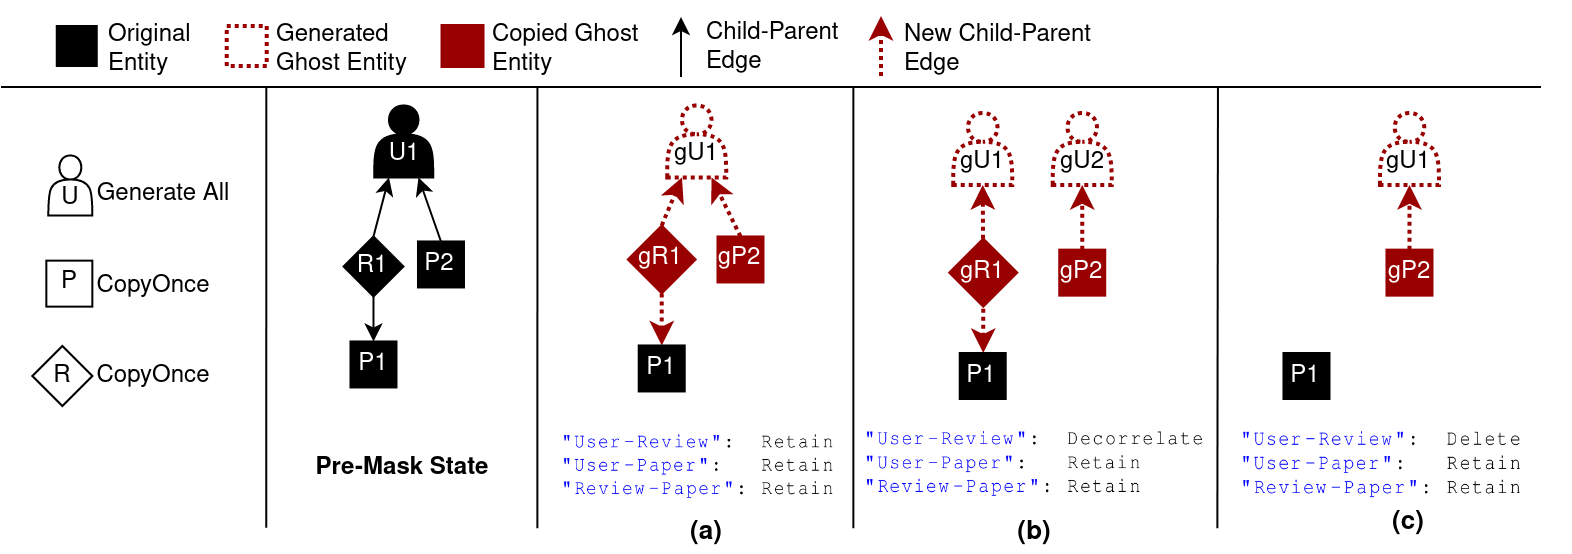
\includegraphics[width=\textwidth]{img/edge_transforms}

    \iffalse
\begin{lstlisting}[language=Rust]
"User-Review":  Retain
"User-Paper":   Retain
"Review-Paper": Retain
\end{lstlisting}

\begin{lstlisting}[language=Rust]
"User-Review":  Decorrelate
"User-Paper":   Retain
"Review-Paper": Retain
\end{lstlisting}

\begin{lstlisting}[language=Rust]
"User-Review":  Delete
"User-Paper":   Retain
"Review-Paper": Retain
\end{lstlisting}
\fi

    \caption{Different edge transformations in the entity graph. User entities are generated and
    paper and review entities are cloned once to retain their content in the application. 
    For clarity, we show only relevant parts of the entity graph and the mask policy, and use entity-granularity ghosting
        transformations rather than per-attribute ones.\\
    \textbf{(a)} retains User-Review edges;
    \textbf{(b)} decorrelates User-Review edges, creating a new ghost user for R1 and rewriting R1's 
    foreign key to point to the new ghost user;
    \textbf{(c)} deletes User-Review edges.\\
    All edge transformations replace all sensitive entities (U1, R1, and P2) with ghost entities.
    }
    \label{fig:edgepol}
\end{figure*}

\begin{figure}[t!]
    \centering
    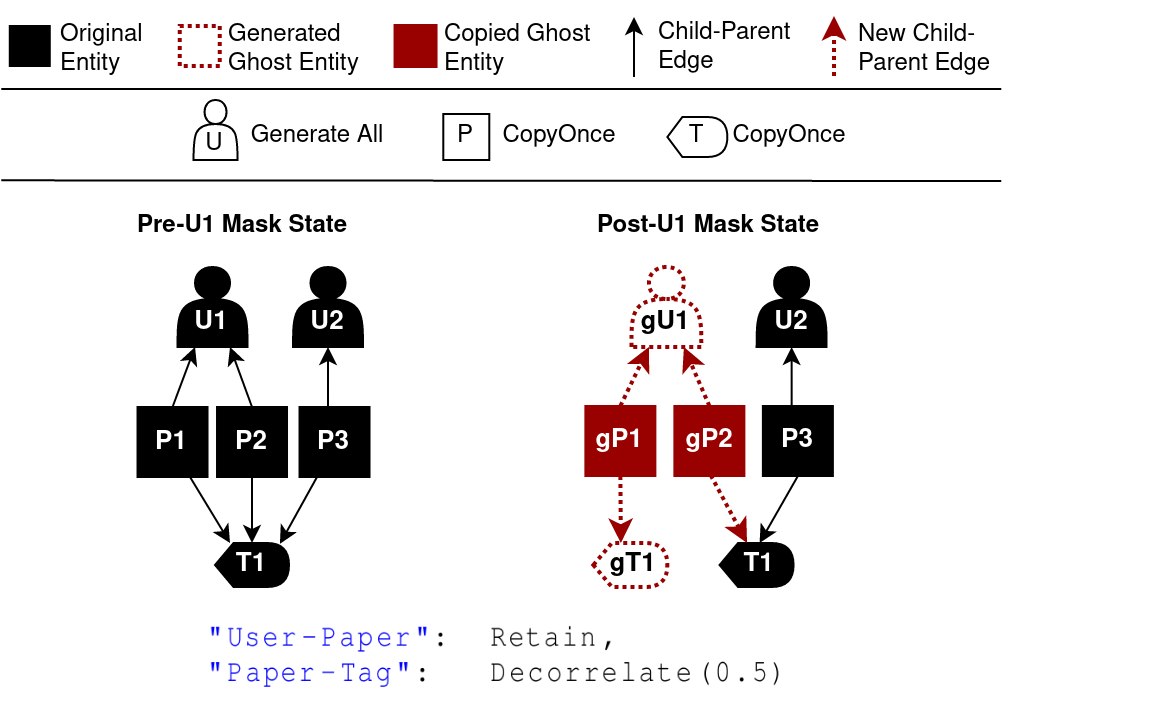
\includegraphics[width=0.54\textwidth]{img/child-parent}

    \iffalse
\begin{lstlisting}[language=Rust]
"User-Paper":  Retain,
"Paper-Tag":   Decorrelate(0.5) 
\end{lstlisting}
\fi

    \caption{An example of a decorrelation edge transformation that decorrelates papers from tags
    until at most 50\% of all papers with the tag are sensitive.
    }
    \label{fig:sensitivity}
\end{figure}

While entity type transformations specify how to create ghost entities, edge transformations 
specify how ghosts restructure the entity graph.

By default, \sys replaces all \emph{sensitive} entities---entities transitively connected via foreign key
relationships (edges in the graph) to the mask's target entity---with ghost entities.
For example, in Figure~\ref{fig:edgepol}a, all reviews and papers of the unsubscribing user are by
default replaced by ghosts.

%Any parent of a sensitive child is ghosted as well. This is not actually true; we retain the
%original parent entity, but allow it to be decorrelated
%\lyt{Child-to-Parent edges can have different ghost
%generation policies + edge policies than Parent-to-Child edges. I'm not sure if we should mention
%that here (seems too detailed?)}

The developer specifies transformations for each parent-child edge type, choosing from the following:
\begin{enumerate}
    \item \textbf{Retain} edges from sensitive children to the parent. Figure~\ref{fig:edgepol}a
        shows how the entity graph is transformed when all edges are retained; \sys ghosts
        sensitive entities according to the specified entity transformation.
    \item \textbf{Decorrelate} edges from sensitive children by replacing edges to the parent with
        ones to a unique ghost parent, generated using the parent as a template:
        child edge attribute values will identify unique ghost parents (Figure~\ref{fig:edgepol}b).
    \item \textbf{Delete} edges from sensitive children by removing the child and its descendants
        (Figure~\ref{fig:edgepol}c).
\end{enumerate}

Some policies also need to decorrelate or delete edges from sensitive children to parents that are
not descendants of the user. For example, papers have both tags and users as parents. If an
unsubscribed user authors all papers with a particular tag, the developer may realize that the tag
can reidentify the user, and want to decorrelate the paper from the tag.

\sys supports these transformations on child-parent edge types, in which developers specify  a
\emph{sensitivity threshold}. This threshold sets the allowable proportion of correlations to
sensitive entities. The developer chooses whether to decorrelate or delete edges to meet this
threshold. In the paper-tag example, a reasonable sensitivity threshold might be $0.1$: fewer than
10\% of all papers with a specific tag key should be correlated with an (unsubscribed) user.
Figure~\ref{fig:sensitivity} shows an example in which paper-tag edges are decorrelated to meet a
threshold of 0.5.

\subsection{Data Masks as Privacy Transformations}
This menu of transformations can describe masks for the range of current and possible privacy
transformations from Section~\ref{sec:survey}. For example, we describe masks for these privacy
transformations as follows:
\begin{itemize}[nosep]
    \item Keep user contributions visible to the intended audience, but anonymized by reassociation with a global
        placeholder user:

        Retain edges from user to contribution entities; transform contribution entities by copying
        entity content, and transform user entities by changing attributes to correspond to the
        global placeholder user attributes (\eg with a username of ``deleted'').

    \item Keep user's contributions, but associate each contribution with a different user account:

        Decorrelate edges from user to contribution entities (\eg posts or reviews);
        transform contribution entities by copying entity
        content. 

    \item Remove users' contributions that have the same public characteristic: 

        Delete edges from
        contribution entity to characteristic entity (\eg papers to tags) with sensitivity threshold
        0.

    \item Remove users' contributions that have the same public characteristic, but only if this
        characteristic was created by the user: 

        Delete edges from characteristic entity to constribution entity (\eg tags to papers).

    \item Ungroup users' contributions that have the same public characteristic, but only if this
        characteristic was created by the user: 

        Decorrelate edges from characteristic entity to constribution entity (\eg tags to papers);
        ghost characteristic entities can be generated as some default placeholder entity (\eg ``untagged'') or
        as appropriate for the application.

    \item Remove users' contributions if they comprise more than $p$
            percent of the contributions with the same public characteristic:
        
        Delete edges from contribution entity to
        characteristic entity (\eg papers to tags) with sensitivity threshold $p$.
\end{itemize}

%%%%%%%%%%%%%%%%%%%%%%%%%%%%%%%%%%%%%%%%%%%%%%%%%%%%%%%%%%%%%%%%%%%%%%%%%%%%%%%%%%%%%%%%%%%%%%%%%%%%%%
%%%%%%%%%%%%%%%%%%%%%%%%%%%%%%%%%%%%%%%%%%%%%%%%%%%%%%%%%%%%%%%%%%%%%%%%%%%%%%%%%%%%%%%%%%%%%%%%%%%%%%
%%%%%%%%%%%%%%%%%%%%%%%%%%%%%%%%%%%%%%%%%%%%%%%%%%%%%%%%%%%%%%%%%%%%%%%%%%%%%%%%%%%%%%%%%%%%%%%%%%%%%%

\iffalse
\sys also handles user data management and storage.
While unsubscribing a user, \sys tracks all deletions and modifications to the database.
\sys encrypts this log with a per-user key, and stores this encrypted
blob in a dedicated application datastore (Figure~\ref{fig:arch}, step 5). The user key is secret-shared using a (2, 3)
threshold scheme~\cite{secretsharing} between the user, \sys, and a trusted third party (\eg
Amazon S3), so that the user can authorize \sys and the third party to restore the key if
the user forgets their share.
%Alternatively, the key can also be password-encrypted, which relies
%on the user not forgetting their password.
The user can optionally choose to store this encrypted data themselves
%(or in a third party cloud provider),
and be in charge of providing their data and key to \sys to decrypt the data upon
resubscription.

To resubscribe, a user authorizes the decryption of their data and associated metadata by
providing their share of the key (or authorizing a trusted third party to reconstruct the secret
with the application). \sys decrypts the data with the key, and systematically reverses
the modifications made during unsubscription, restoring removed entities and correlations between
entities.
\fi

%%%%%%%%%%%%%%%%%%%%%%%%%%%%%%%%%%%%%%%%%%%%%%%%%%%%%%%%%%%%%%%%%%%%%%%%%%%%%%%%%%%%%%%%%%%%%%%%%%%%%%
%%%%%%%%%%%%%%%%%%%%%%%%%%%%%%%%%%%%%%%%%%%%%%%%%%%%%%%%%%%%%%%%%%%%%%%%%%%%%%%%%%%%%%%%%%%%%%%%%%%%%%
%%%%%%%%%%%%%%%%%%%%%%%%%%%%%%%%%%%%%%%%%%%%%%%%%%%%%%%%%%%%%%%%%%%%%%%%%%%%%%%%%%%%%%%%%%%%%%%%%%%%%%

\iffalse
\subsection{\sys's Execution Algorithm}
\begin{figure*}[ht!]
    \centering
    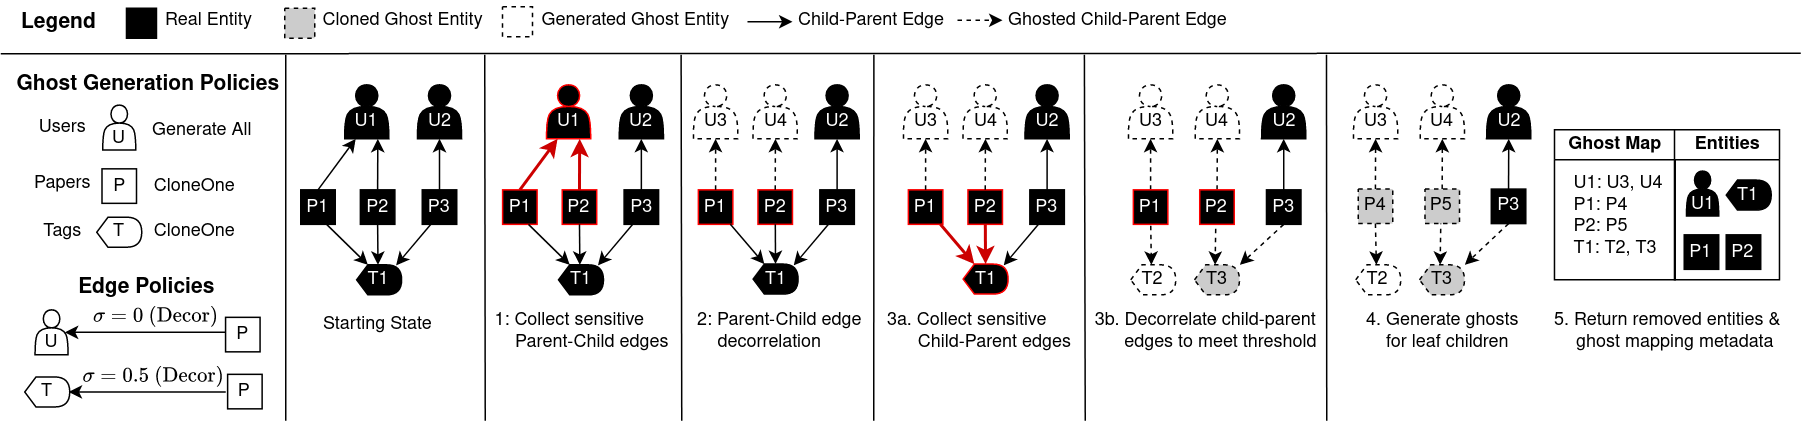
\includegraphics[width=\textwidth]{img/algo}

    \caption{Stages of \sys's execution when unsubscribing user U1. Entities and edges detected as
    sensitive are outlined in red. Only the part of the entity graph relevant to unsubscription is shown.
    For simplicity, the specified ghosting policies apply for all attributes
    of the entity: a black ghost entity indicates that it is a full clone of the original.
    New edges indicates that the edge (foreign-key) value of the child has been changed to
    point to the specified parent.\\
    In this example, \sys decorrelates paper-tag edges only enough that the proportion of sensitive papers
    is at most the sensitivity threshold of 0.5, retaining one correlation between a sensitive
    paper P2 and the parent tag T1, and decorrelating the other sensitive paper P1 from the tag.}
    \label{fig:algo}
\end{figure*}


Given an application's schema and unsubscription policy, and an entity to be decorrelated as input,
\sys executes unsubscription as follows. Figure~\ref{fig:algo} illustrates each step.
\begin{enumerate}
    \item \textbf{Parent-Child Traversal:} \sys traverses the entity graph starting from the input entity,
        going down parent to child edges (and halting if it detects a cycle).
        \sys collects traversed edges as it traverses the graph.

    \item \textbf{Parent-Child Edge Policy Application:}
        Post-traversal, \sys acts on each collected edge instance according to the specified
        decorrelation relationship policy for that edge's type.

        \sys takes all edges of every unique parent entity, and applies policies as appropriate.
        Note that any sensitivity threshold less than $1$ requires that \emph{all} edges be decorrelated or
        deleted, depending on the developer's specified choice: all the children of this parent are
        sensitive due to the nature of \sys's parent-child traversal.

        Any edges that should be deleted removes the child entity and any descendants.
        \sys generates new ghost parents using the real parent as template for any edges that should
        be decorrelated, and rewrites the child's edge attribute to be the ghost parent's
        identifier. If any edges are retained, \sys generates a ghost parent entity to replace the
        parent.

    \item \textbf{Child-Parent Edge Policy Application:}
        Next, \sys takes the children of all traversed edge instances, and considers the set of
        edges from these children to other parents \emph{not} traversed by \sys during the first
        traversal phase. In other words, these children have multiple parents, at least one of which
        is transitively connected to the input entity.

        Intuitively, children of edges traversed by \sys share a connection with the initial
        entity being decorrelated. Edges \emph{from} these children to other parent entities may
        thus leak sensitive identifying information.

        \sys acts on these child-parent edges according to the specified edge policy for each edge's
        type. For each unique parent, \sys limits the proportion of edges of each type that connect
        to sensitive entities (the children of traversed edge instances) to below the policy's
        sensitivity threshold by either decorrelating or deleting the children.
        If \sys retains any edges from sensitive children to the real parent, then \sys generates a
        ghost parent entity to replace the parent.

        Note that unlike the previous steps, this step considers edges from parents that may have
        many non-sensitive children (\eg a particular tag may correlate with many stories by various
        authors).  \sys therefore may retain edges to sensitive children when given a sensitivity
        threshold less than 1 and greater than 0, unlike in the previous step.

        \sys optionally allows developers to specify that edges have weaker or stronger edge
        policies in the child-to-parent direction than in the  parent-to-child direction. Weaker
        policies---higher sensitivity thresholds---allow \sys to retain links if \emph{only the
        child} is sensitive, but decorrelate or remove the link if \emph{both} the child and parent
        are sensitive. For example, perhaps a user wants to ensure that they are decorrelated from
        their reviews, but correlations between the review and the the paper authors can still be
        retained.

        Stronger policies may specify that the parent connected to sensitive children should
        decorrelate \emph{all} correlations to the paper even from non-sensitive correlations.
        Developers specify such a policy with a sensitive threshold of -1. For
        example, perhaps the set of users with review conflicts to the paper can identify the
        author, even if the author is decorrelated from the paper. We see an example of this in
        Section~\ref{sec:hotcrp_example} (Figure~\ref{fig:pcs}).

    \item \textbf{Anonymizing Leaf Children:}
        If any sensitive children that are leaves (have no children) remain, \sys generates a ghost child entity to replace this leaf.

        In Figure~\ref{fig:algo}, step 4, P1 and P2 are both leaves. \sys generates ghosts for both
        these papers: since these papers have \texttt{CloneOne} ghosting policies, ghost papers gP1
        and gP2 are identical to P1 and P2, and retain the edge attributes linking them to their
        respective parent tags and users.

    \item \textbf{Returning User Data:} \sys collects all removed entities that have either been
        replaced by ghost entities, or deleted entirely from the graph. \sys also records all
        generated ghost entity identifiers, and which ghost entities replaced which real entity.
        \sys returns both the removed entity data and this ghost entity metadata to the user.
\end{enumerate}

Note that \sys must decide \emph{which} ghost clones the template entity's attributes when the
developer selects a \texttt{CloneOne} ghosting policy for one or more attributes. \sys always
associates the cloned ghost with as many non-sensitive entities as possible. For example, as shown
in Figure~\ref{fig:algo} step 3b, if \sys decorrelates sensitive papers from a parent tag with a
\texttt{CloneOne} policy, \sys chooses the ghost tag that remains associated with non-sensitive
papers to be the clone. This decision ensures that any unsensitive application
data remain as unaffected as possible when masking another entity.
To optimize
\texttt{CloneOne} policies, \sys can simply retain the original template entity instead of producing
a cloned ghost.
\fi
%\sys provides a menu of unsubscription policy choices that allow developers to choose how to
%\emph{ghost} individual data record content, and how to \emph{decorrelate} sensitive correlations.
%Specifying the policy requires nothing more than the application schema: ghosting policies act on
%application datatables and on foreign key relationships between tables.
%Table column values can be ghosted---removed, anonymized, or modified---in application-specific
%ways; and correlations can be broken, removed, or desensitized by adding noise. This gives
%developers the flexibility to specify fine-grained policies that properly de-identify a user, while
%retaining data as necessary for the application.

%\sys must pinpoint exactly which data and correlations may be
%identity-sensitive, and allow developers to specify exactly what the post-unsubscription state of
%this data should be.


